\documentclass[12pt,a4paper]{article}
\usepackage[a4paper]{geometry}
\usepackage[utf8]{inputenc}
\usepackage[english]{babel}
\usepackage{amsmath}
\usepackage{amsfonts}
\usepackage{amssymb}
\usepackage{graphicx}
\author{Ethan Kelly}
\title{The Network $SIRP$ Model}
\begin{document}

\maketitle

\section{Equations}

\subsection{Standard $SIR$ model with fixed population}

The SIR Model is a compartmental epidemiological model with three compartments (generally referred to as `states') related to an epidemic: {\it susceptible, infected} and {\it recovered.} We define $S(t)$ as the number of people who do not currently have but are able to contract the infection at time $t$, $I(t)$ as individuals who currently have the disease and are infectious and finally $R(t)$ as those who have had the disease and subsequently recovered, granting them at least some level of immunity in certain contexts. For a fixed population $N$, we have that $S(t) + I(t) + R(t) = N$ - that is, we assume a fixed population where we do not wish to consider vital dynamics, usually when an epidemic is short-lived. Then, for $\beta$ and $\gamma$ the rates of infection and recovery respectively, the standard SIR model without vital dynamics (birth and death rates) is given as follows:

\begin{align}
\frac{dS}{dt} & = -\beta \frac{SI}{N} \label{dS}\\
\frac{dI}{dt} & = \beta\frac{SI}{N} \gamma I \label{dI}\\
\frac{dR}{dt} & = \gamma I - \mu R \label{dR}
\end{align}

We generally aren't much interested in the expression for $\dot{\langle R \rangle}$, since we require that $ \dot{\langle S \rangle} + \dot{\langle I \rangle} + \dot{\langle R \rangle} = 1$ meaning we can always find the third probability as the compliment of the sum of the other two probabilities. In much of the literature, the convention is for this reason to only give the first two equations.

\subsection{Extending the $SIR$ model to networks}

In order to extend our SIR model to network models, we first examine the probability of an agent being in a given class: let $\langle A_i \rangle$ represent the time-independent probability of person $i$ being in state $A$, meaning that the expression of the form $\langle A_i B_i \rangle$ represents the (again, time-independent) probability of individuals $i$ and $j$ being in states $A$ and $B$ respectively \cite{kiss15}. We begin with a contact network, where vertices represent individuals and the edges between them represent social contact which may serve as an infection pathway. Then, the adjacency matrix $G$ of this network is constructed by assigning $G_{ij} = 1$ when $i$ and $j$ share an edge and $G_{ij} = 0$ otherwise.\footnote{Because we are infrequently interested in self-transmission, we often set $G_{ii}=0.$} Then, we extend this contact network to a transmission network: let $\beta_i$ represent the per-link infection rate for individual $i$ and $\gamma_i$ represent the recovery rate for $i$. For the transmission matrix $T,$ we assign $T_{ij}=\beta_i$ if there is a route of infection between $i$ and $j$ and $T_{ij}=0$ otherwise. Often, we will consider unweighted and undirected graphs, but in general $T_{ij}$ may not equal $T_{ji}$.\\
We now note that we can replace $\beta_i$ with a term involving such a transmission matrix of a network in order to begin extending the usual SIR model into a network realm. Using the substitution $ \beta_i \frac{SI}{N} = \sum^{N}_{j=1}T_{ij} \langle S_i I_j \rangle,$ the equations become
\begin{align*}
\dot{\langle S_i \rangle} & = -\sum^{N}_{j=1}T_{ij} \langle S_i I_j \rangle\\
\dot{\langle I_i \rangle} & =\sum^{N}_{j=1}T_{ij}\langle S_i I_j \rangle - \gamma_i \langle I \rangle \\
\dot{\langle R_i \rangle} & = \gamma_i \langle I \rangle,
\end{align*}
which are the evolution equations given in \cite{kiss15}.

\section{Protection}

\subsection{Adding a new state to the model}

Let $\zeta_i$ be the probability that we defend individual $i$. This can be determined in a number of different ways and we propose that a good candidate for this would be an algorithmic approach.\footnote{That is, determine the best candidates for defence each turn and distribute some given probability across them by the expected benefit in containing the infection gained by defending each vertex.} Similarly, let $\alpha_i$ represent the efficacy of the protection measure for individual $i$, which may decay over time and vary from person to person (for instance, the protection could be more effective in certain age groups than in others). Using these rates of protection and effectiveness, for fixed population size the differential equations become:
\begin{align}
\dot{\langle S_i \rangle} & = \alpha_i \langle P_i \rangle - \sum^{N}_{j=1}T_{ij} \langle S_i I_j \rangle - \zeta_i\langle S_i \rangle\\
\dot{\langle I \rangle} & =\sum^{N}_{j=1}T_{ij}\langle S_i I_j \rangle - \gamma_i \langle I \rangle \\
\dot{\langle R_i \rangle} & = \gamma_i \langle I \rangle \\
\dot{\langle P_i \rangle} & = \zeta_i \langle S_i \rangle - \alpha_i \langle P_i \rangle.
\end{align} 
Accounting for vital dynamics, with a birth and death rate (for simplicity) of $\mu$, these equations are:
\begin{align}
\dot{\langle S_i \rangle} & = \alpha_i \langle P_i \rangle - \sum^{N}_{j=1}T_{ij} \langle S_i I_j \rangle + \mu N - \mu \langle S_i \rangle - \zeta_i\langle S_i \rangle\\
\dot{\langle I \rangle} & =\sum^{N}_{j=1}T_{ij}\langle S_i I_j \rangle - \gamma_i \langle I \rangle - \mu \langle I_i \rangle\\
\dot{\langle R_i \rangle} & = \gamma_i \langle I \rangle + \mu \langle R_i \rangle\\
\dot{\langle P_i \rangle} & = \zeta_i \langle S_i \rangle - \alpha_i \langle P_i \rangle - \mu \langle P_i \rangle.
\end{align}

\subsection{Results for total system of equations}

As an example, we consider the `triangle network.' This is a loop of three nodes and the equations required to precisely express the system $SIR$ dynamics of this network are as follows \cite{kiss15}:
\begin{align}
\text{6 singles: } & \dot{\langle S_1 \rangle}, \dot{\langle S_2 \rangle}, \dot{\langle S_3 \rangle}, \dot{\langle I_1 \rangle}, \dot{\langle I_2 \rangle}, \dot{\langle I_3 \rangle}.\label{eq:SIRsingle}\\
\text{6 doubles: } & \dot{\langle S_1 I_2 \rangle},\dot{\langle I_1 S_2 \rangle}, \dot{\langle S_1 I_3 \rangle}, \dot{\langle I_1 S_3 \rangle}, \dot{\langle S_2 I_3\rangle}, \dot{\langle I_2 S_3 \rangle}.\label{eq:SIRdouble}\\
\text{6 triples: } & \dot{\langle S_1 I_2 I_3 \rangle}, \dot{\langle S_1 I_2 S_3 \rangle}, \dot{\langle S_1 S_2 I_3 \rangle}, \dot{\langle I_1 S_2 S_3 \rangle}, \dot{\langle I_1 I_2 S_3 \rangle}, \dot{\langle I_1 S_2 I_3 \rangle}. \label{eq:SIRtriple}
\end{align}
Now, using the equations for the $SIRP$ model, we have the following equation requirements:
\begin{align*}
\text{9 singles: (} \ref{eq:SIRsingle} \text{) and } & \dot{\langle P_1 \rangle}, \dot{\langle P_2 \rangle}, \dot{\langle P_3 \rangle}.\\
\text{18 doubles: (} \ref{eq:SIRdouble} \text{) and }& \dot{\langle S_1 P_2 \rangle},\dot{\langle P_1 S_2 \rangle}, \dot{\langle I_1 P_2 \rangle}, \dot{\langle P_1 I_2 \rangle}, \dot{\langle S_1 P_3\rangle}, \dot{\langle P_1 S_3 \rangle},\\ & \dot{\langle I_1 P_3 \rangle}, \dot{\langle P_1 I_3 \rangle}, \dot{\langle S_2 P_3 \rangle}, \dot{\langle P_2 S_3 \rangle}, \dot{\langle I_2 P_3 \rangle}, \dot{\langle P_2 I_3 \rangle}. \\
\text{24 triples: (} \ref{eq:SIRtriple} \text{) and } & \dot{\langle S_1 S_2 P_3 \rangle}, \dot{\langle S_1 P_2 S_3 \rangle}, \dot{\langle S_1 I_2 P_3\rangle}, \dot{\langle S_1 P_2 I_3 \rangle}, \dot{\langle S_1 P_2 P_3\rangle}, \dot{\langle I_1 S_2 P_3 \rangle},\\
&  \dot{\langle I_1 P_2 S_3 \rangle}, \dot{\langle I_1 I_2 P_3 \rangle}, \dot{\langle I_1 P_2 I_3 \rangle}, \dot{\langle I_1 P_2 P_2 \rangle},  \dot{\langle P_1 S_2 S_3 \rangle}, \dot{\langle P_1 S_2 I_3 \rangle},\\
&  \dot{\langle P_1 I_2 S_3 \rangle}, \dot{\langle P_1 I_2 I_3 \rangle}, \dot{\langle P_1 P_2 I_3 \rangle},  \dot{\langle P_1 P_2 S_3 \rangle}, \dot{\langle P_1 S_2 P_3 \rangle},  \dot{\langle P_1 I_2 P_3\rangle}.
\end{align*}


Note that the reason we dispense with the cases of all three vertices being in the same state is that this would not result in any dynamics - no vertices would ever change state in this case. 

\newpage

\section{Equation generation: Algorithmic approach}

\begin{figure}[!ht]
\centering
     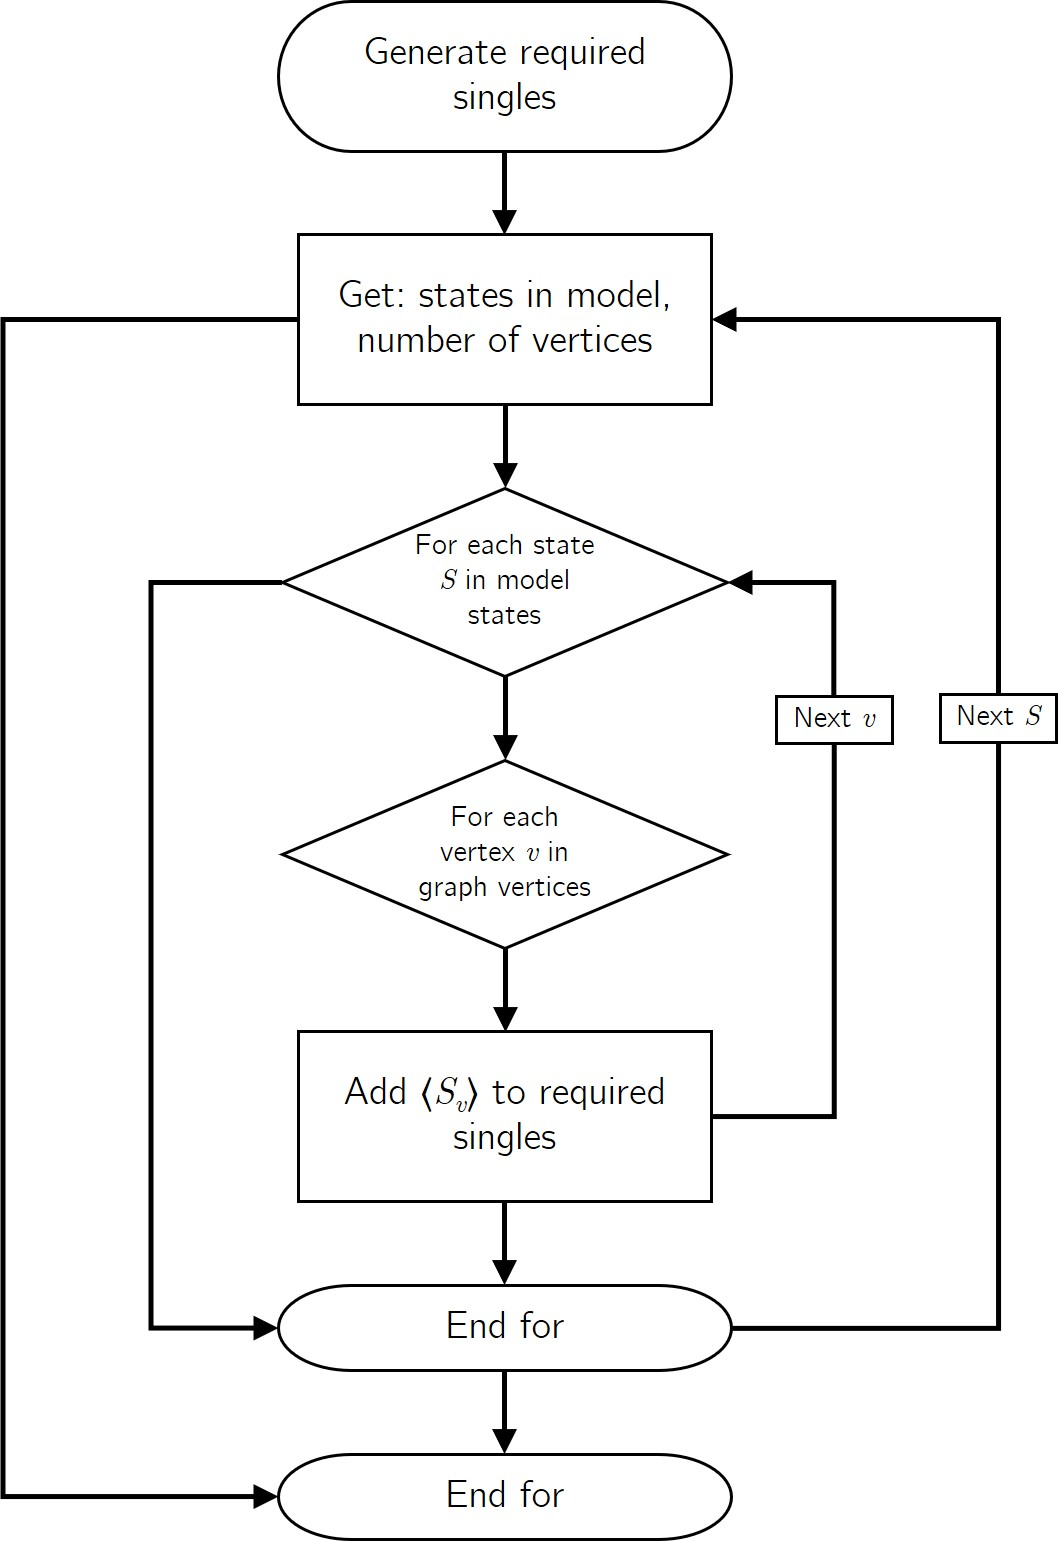
\includegraphics[width=0.85\textwidth]{Equations/GenerateSingles}
         \caption{Singles Generation Flowchart}
         \label{fig:gen-singles}
\end{figure}

\begin{figure}[!ht]
\centering
     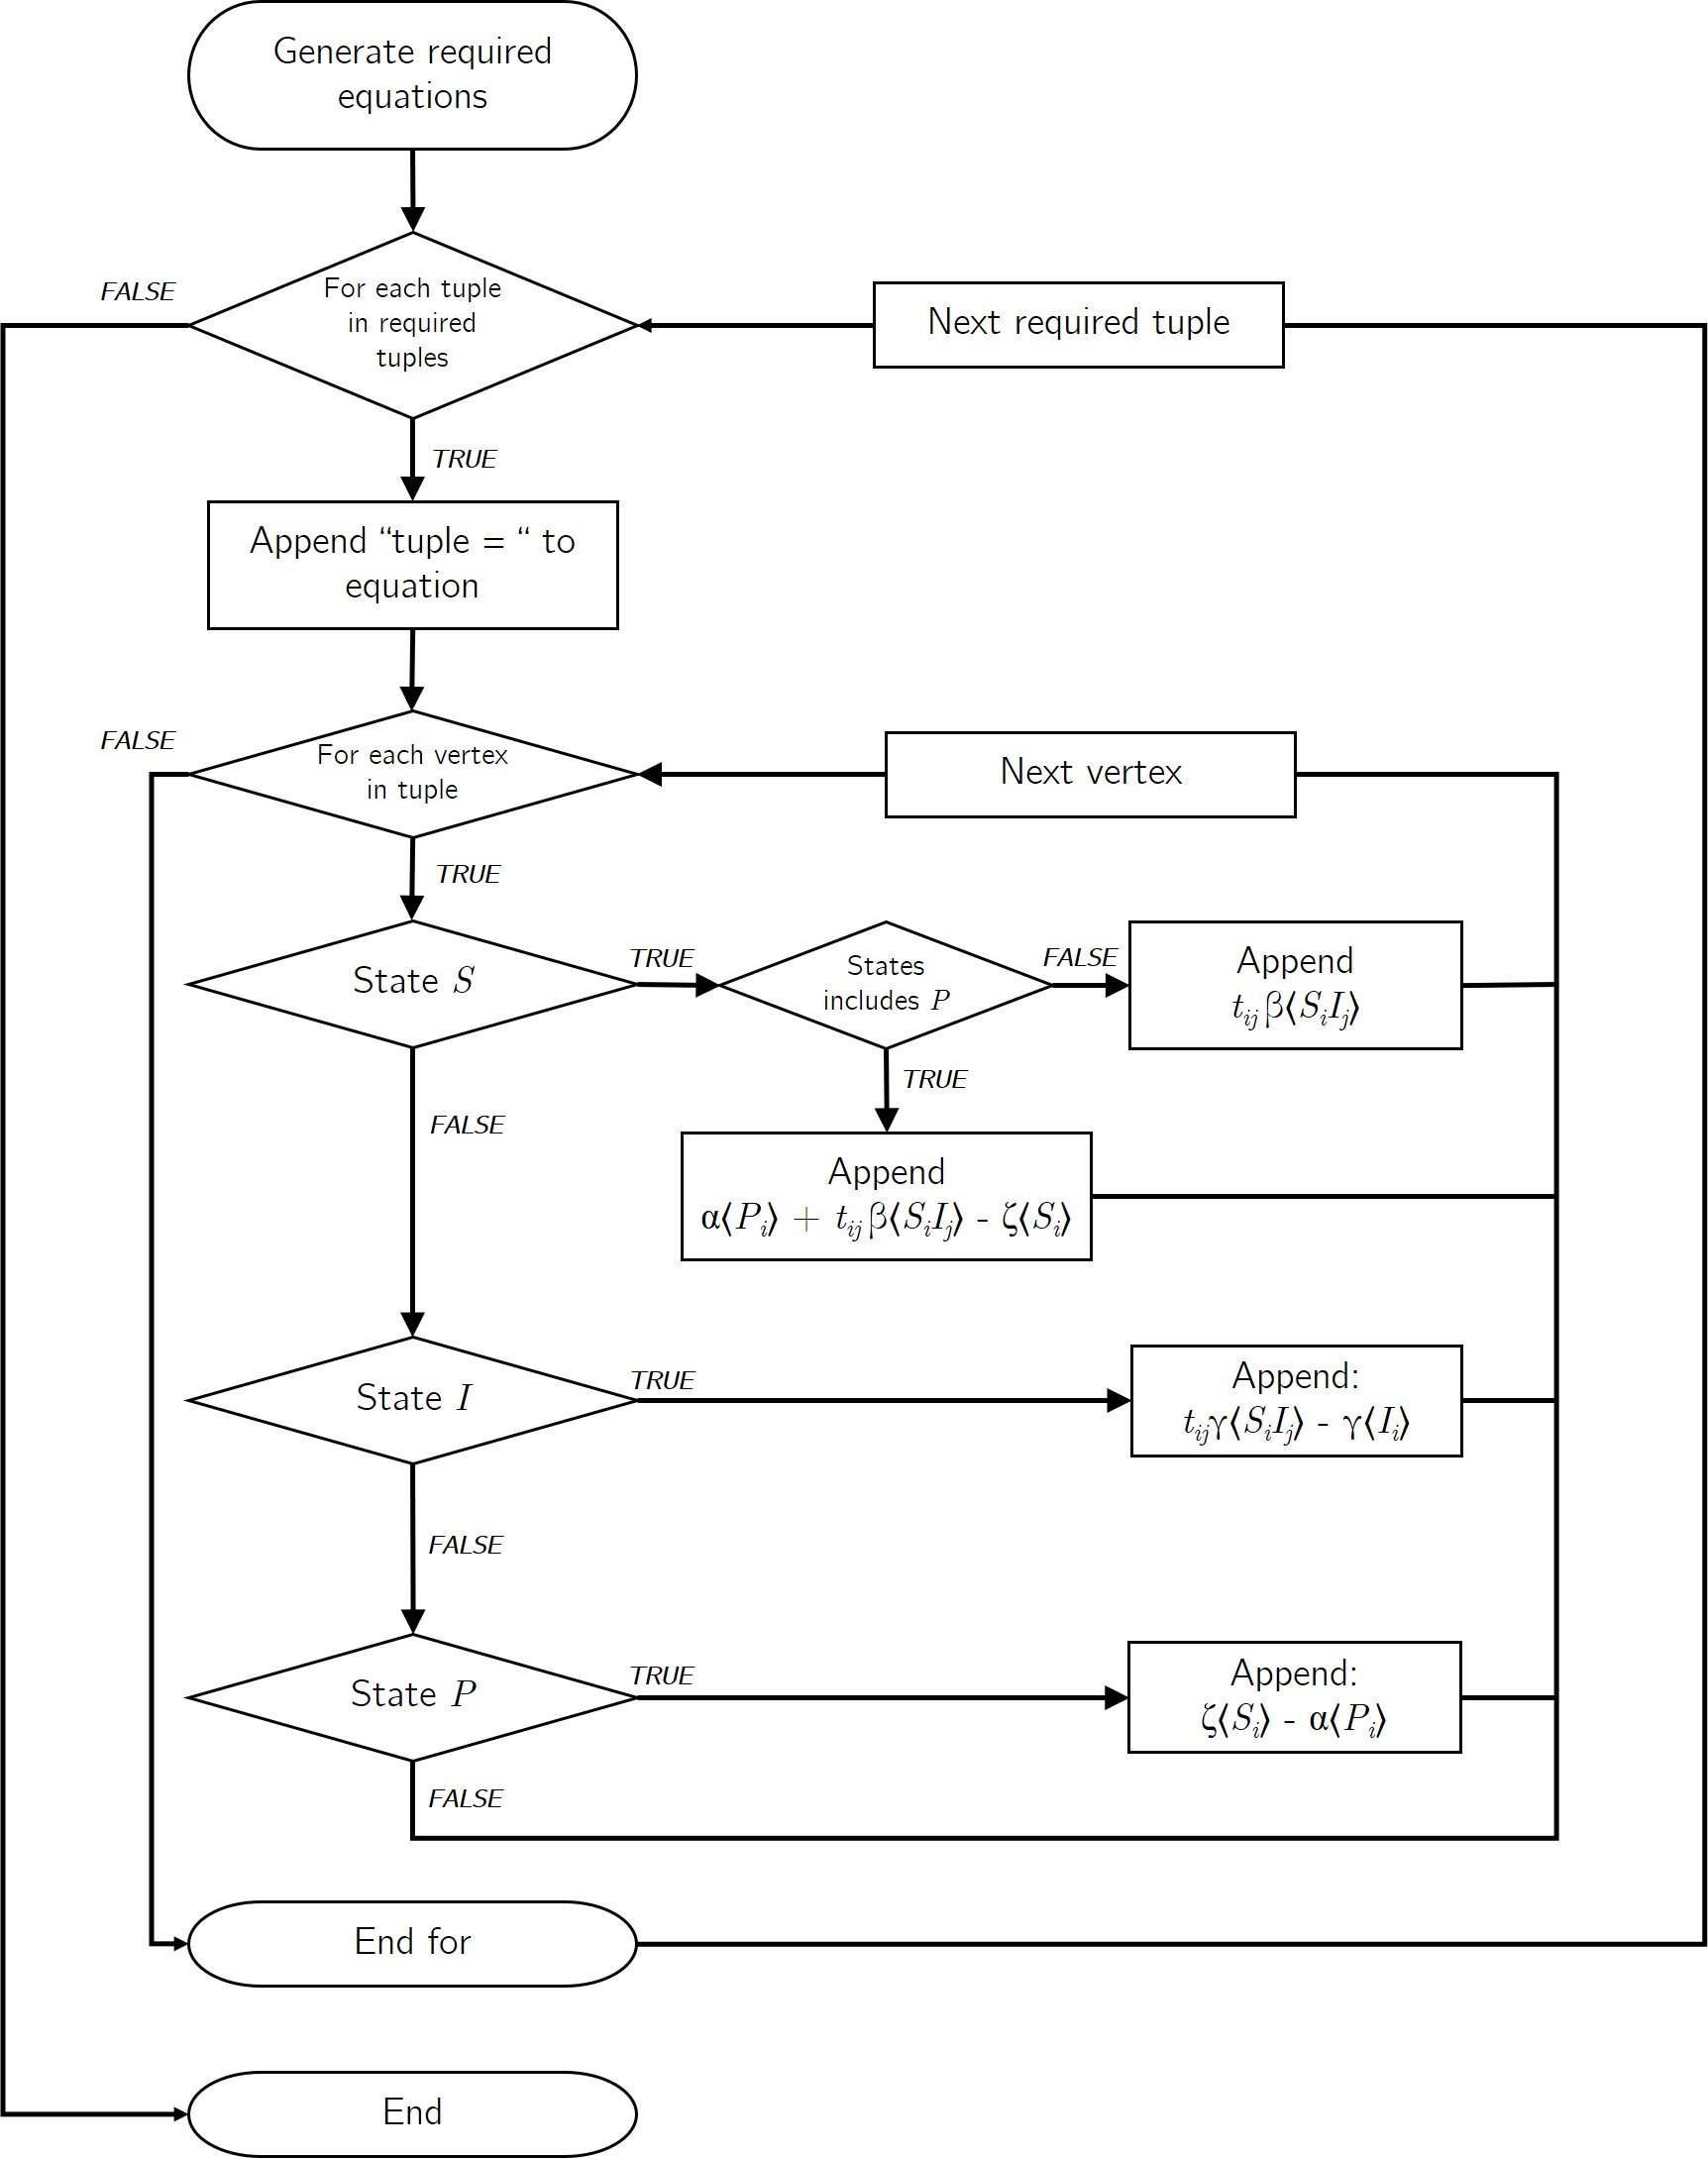
\includegraphics[width=0.9\textwidth]{Equations/GenerateEquations}
         \caption{Singles Generation Flowchart}
         \label{fig:gen-singles}
\end{figure}


\newpage
\bibliographystyle{siam}
\bibliography{bibliography}

\end{document}
